
\section{Adaptive tabu search (ATS)}
\textit{Katarzyna Śmietanka, Tomasz Dziopa}
\subsection{Rozszerzenie sformułowania problemu }
Rozszerzenie specyfikacji problemu z sekcji 3.2.4.
\par Problem definiujemy w postaci macierzy ${X}$  rozmiaru ${p \times m}$ gdzie ${x_{i,j}}$ ($x$ - unikalna etykieta zajęć) definiuje przypisanie danych zajęć do ${t_{j}}$ okresu oraz sali ${r_{i}}$. Jeżeli w danym czasie w danej sali nie odbywają się zajęcia wartość ${x_{i,j}}$ będzie przyjmowała wartość ${null}$. Dzięki takiemu sposobowi zdefiniowania problemu nigdy nie zostanie naruszone ograniczenie twarde ${H_{2}}$ dotyczące zajętości sali.

\begin{table}[H]
\begin{center}

\begin{tabular}{ r|c|c|c|c|c| }
\multicolumn{1}{r}{}
 &  \multicolumn{1}{c}{$r_{1}$}
 & \multicolumn{1}{c}{$r_{2}$} 
 & \multicolumn{1}{c}{$r_{3}$} 
 & \multicolumn{1}{c}{$...$} 
 & \multicolumn{1}{c}{$r_{m}$} 
 \\
\cline{2-6}
$t_{1}$ & $null$ & $matematyka$ & $biologia$ & $...$ & $geografia$ \\
\cline{2-6}
$t_{2}$ & $fizyka$ & $null$  & $null$ & $...$ & $religia$\\
\cline{2-6}
$t_{3}$ & $historia$ & $null$  & $null$ & $...$ & $null$\\
\cline{2-6}
$...$ & $...$ & $...$ & $...$ & $...$ & $...$ \\
\cline{2-6}
$t_{p}$ & $null$ & $matematyka$ & $chemia$ & $...$ & $fizyka$ \\
\cline{2-6}
\end{tabular}
\end{center}
\caption {Reprezentacja problemu w postaci macierzy $X$}
\end{table} 
\begin{itemize}
 \item Komórka $(t_{2}, r_{2}) = null$ w macierzy $X$ oznacza, że w czasie $t_{2}$ w sali $r_{2}$ nie odbywają się żadne zajęcia.
 \item Komórka $(t_{3}, r_{1}) = historia$ w macierzy $X$ oznacza, że w czasie $t_{3}$ w sali $r_{1}$ odbywają się zajęcia z przedmiotu $historia$.
\end{itemize}


\subsection{Ogólny opis algorytmu}
\par Opis zaimplementowanego przez nas algorytmu został zaczerpnięty z pracy ,,Adaptive TabuSearch for Course Timetabling'' \cite{tabu}
\par Na całość algorytmu składają się trzy fazy: faza inicjalizacji podczas której tworzony jest początkowy plan zajęć, przy pomocy zachłannej heurystyki, faza intensyfikacji, która jest właściwą fazą algorytmu Adaptive Tabu Search, której celem jest optymalizacja funkcji oceny ograniczeń miękkich. Końcowa faza - faza dywersyfikacji gdzie dokonywana jest redukcja naruszeń miękkich, tak aby nie łamać twardych ograniczeń. Na algorytm ten składa się wiele unikalnych cech między innymi struktury sąsiedztwa - podwójne łańcuchy Kempe, operator zaburzeń oraz dynamiczna integracja operacji przeszukiwania tabu z operatorem zaburzeń.

\subsection{Tabu Search}
\par Algorytm Tabu Search został zaprezentowany w 1986 roku przez Freda W. Glovera \cite{glover}. Jest to metaheurystyka, która opiera się na obserwacji, że proces przeszukiwania przestrzeni rozwiązań w poszukiwaniu najlepszego u ludzi i zwierząt opiera się na pamięci krótko- i długoterminowej. 
\par Pamięć krótkoterminowa realizowana jest w postaci listy ruchów zabronionych. W każdej iteracji przeglądamy strukturę sąsiedztwa w poszukiwaniu najlepszego rozwiązania. Sprawdzamy, czy ruch prowadzący do uzyskania najlepszego sąsiada nie znajduje się na liście ruchów zabronionych; jeżeli tak - rozważamy kolejnego najlepszego sąsiada, w przeciwnym wypadku - aktualizujemy rozwiązanie i dodajemy ruch prowadzący do niego jako ruch zabroniony.

\begin{algorithm}[H]
    \caption{Algorytm Tabu Search}
    \begin{algorithmic}
    \STATE{$rozwiazanie_{najlepsze} = rozwiazanie_{aktualne}$}
    \WHILE{\emph{nie jest spełniony warunek stopu}}
    \STATE{$sąsiedztwo = oblicz\_sąsiedztwo(rozwiazanie_{aktualne})$}
    \FOR{$i=0$ \TO len($sąsiedztwo$)}
    	\IF{$ruch(rozwiazanie_{aktualne}, sąsiedztwo[i]) \not \in lista\_tabu$}
    	\STATE $lista\_tabu = lista\_tabu \cup ruch(rozwiazanie_{aktualne}, sąsiedztwo[i])$
    	\STATE $rozwiazanie_{aktualne} = sąsiedztwo[i]$
    	\ENDIF
    	\IF{$jakość(rozwiazanie_{aktualne})<jakość(rozwiazanie_{najlepsze} )$}
    	\STATE $rozwiazanie_{najlepsze} = rozwiazanie_{aktualne}$
    	\ENDIF
    	
    \ENDFOR
    \ENDWHILE
    \end{algorithmic}
    \end{algorithm}

\subsection{Fazy algorytmu}
\subsubsection{Faza inicjalizacji}
\par W tej fazie tworzony jest wykonywalny plan zajęć czyli nienaruszający ograniczeń twardych ${H_{1} - H_{4}}$. W każdej iteracji wybierane jest jedno z zajęć z kursu i przypisywane do odpowiedniego okresu i pomieszczenia. Całość przydzielania odbywa się na podstawie dwóch heurystyk pierwsza z nich determinuje wybor kursu, który zostanie przypisany do planu zajęć oraz druga zaś określa parę okres-sala.
\par Dla każdego częściowo wykonywalnego planu zajęć ${P}$ (czyli takiego, do którego zostało przydzielone już część zajęć nie naruszając ograniczeń twardych) próbujemy wybrać jedne z zajęć z kursu, który posiada jeszcze nieprzydzielone zajęcia zgodnie z heurystyką ,,Wybór kursu''. Dzięki tej heurystyce uzyskujemy pierwszeństwo w przydzielaniu kursów mających małą liczbę dostępnych okresów do których może być przypisany oraz kursów z dużą liczbą nieprzypisanych zajęć do planu. Druga z heurystyk ,,Wybór okresu'' dotyczy wyboru okresu, do którego zostaną przypisane dane zajęcia. Celem jest wybór takiego okresu, który ma najmniejsze prawdobodobieństwo bycia wybranym w kolejnych krokach, dla kolejnych nieskończonych kursów.

\par \textbf{Oznaczenia}
\begin{enumerate}
\item $ lo_{i}(P)$ - liczba okresów do których mogą być przydzielone zajęcia z kursu $c_{i}$ dla planu ${P}$
\item $ lp_{i}(P)$ - liczba dostępnych par: okres- sala dla kursu ${c_{i}}$ dla planu ${P}$
\item $ lnz_{i}(P)$ - liczba nieprzydzielonych zajęć dla kursu ${c_{i}}$ dla planu ${P}$
\item $ lnk_{i, j}(P)$ - liczba zajęć z nieskończonych kursów, których nie można przydzielić do okresu ${t_{j}}$ po przydzieleniu jednego z zajęć z kursu ${c_{i}}$ do okresu ${t_{i}}$
\item $kom(i, j, k)$ - całkowita kara związana z ograniczeniami miękkimi po wykonalnym wstawieniu zajęć (tzn. nie naruszając ograniczeń $H1 - H4$ ) z kursu $c_{i}$ do okresu ${t_{j}}$ przydzieleniu sali ${r_{k}}$
\item $konf_{i}$ - liczba kursów konfliktujących z kursem $c_{i}$, czyli takich które należą do tego samego programu nauczania co kurs $c_{i}$ lub prowadzone są przez tego samego nauczyciela
\end{enumerate}
\par \textbf{Heurystyki}

\begin{enumerate}
  \item Wybór kursu 
  \begin{enumerate}
    \item Wybieramy kurs z najmniejszą wartością współczynnika:\\
     $ w_a(c_{i}) = \frac{lo_{i}(P)}{\sqrt{lnz_{i}(P)}}$
    \item Jeżeli istnieje więcej niż jeden kurs z tą samą wartością współczynnika ${w_a}$ wybieramy kurs z najmniejszym współczynnikiem \\ $ w_b(c_{i}) = lp_{i}(P) * \sqrt{lnz_{i}(P)} $
    \item Jeżeli istnieje więcej niż jeden kurs z tą samą wartością współczynnika $w_b$ to wybieramy kurs ${c_{i}}$ z maksymalną woarością funkcji $konf_{i}$
 
  \end{enumerate}
  \item Wybór okresu \\
  Dla każdej dostępnej pary (okres - sala) wybieramy parę z najmiejszą wartością funkcji $g(j, k) = K_{1} * lnk_{i,j}(P) + K_{2} * kom(i, j, k)$ \\
  $k_{1} = 1.0 $ - współczynnik związany z ograniczeniami twardymi \\
  $k_{2} = 0.5 $ - współczynnik związany z ograniczeniami miękkimi
\end{enumerate}



\subsubsection{Faza intensyfikacji}
\par W fazie intensyfikacji zostają wprowadzone struktury sąsiedztwa prostego oraz pojedyncze i podwójne łańcuchy Kempe, w obrębie tych struktur dochodzi do zamian poszczególnych zajęć tak by nie naruszyć ograniczeń twardych. Na algorytm Tabu Search składa się kombinacja połączenia zamian w obrębie tych dwóch struktur, które przeprowadzane są w cyklu token - ring. Celem tej fazy jest minimalizacja funkcji kary w taki sposób, by nie zostały złamane żadne ograniczenia twarde. Przestrzeń wykonywanych zamian dla poszczególnych zajęć jest ograniczona tylko do wykonywalnych zamian czyli takich, które po przeprowadzeniu ich nie naruszają ${H1-H4}$.
\paragraph{Struktury sasiedztwa}
\begin{enumerate}
\item \textbf{Podstawowa struktura sąsiedztwa} \\
Jest to struktura, która zawiera wszystkie możliwe zamiany dla pary dwóch zajęć należących do różnych kursów i nie należących do tego samego okresu w planie zajęć. \\
Zamiana jest przypisaniem zajęć $x_{i_{1},j_{1}}$ w miejsce zajęć ${x_{i_{2}, j_{2}}}$ oraz zajęć ${x_{i_{2}, j_{2}}}$ w miejsce zajęć $x_{i_{1},j_{1}}$ \\
Możliwe przypadki zamian

\begin{enumerate}
\item Zamiana pomiędzy dwoma różnymi zajęciami należącymi do dwóch różnych kursów i okresów
\item Przypisanie zajęcia ${x_{i,j}}$ do wolnej pozycji - do okresu dla którego zajęcie ${x_{i,j}}$ nie wchodzi w konflikt z pozostałymi zajęciami w tym okresie (tzn. nie narusza ${H1-H4}$ )
\end{enumerate}
Przykład możliwych zamian dla podstawowej struktury sąsiedztwa na podstawie zdefiniowanego poniżej problemu (format danych wejściowych zdefiniowany w sekcji 3.2.5, tutaj stosujemy uproszczoną wersję pomijając niektóre parametry nieistotne w tej fazie):
\begin{alltt}
Dane wejściowe:
Kursy: 
biologia n1 1
fizyka n2 1
matematyka n3 1
język polski n4 1
język angielski n5 2
historia n6 1
religia n7 1
etyka n8 1
Sale: 
sala1
sala2
sala3
sala4
Programy nauczania:
Program1 3 biologia fizyka matematyka
Program2 3 język polski język angielski historia
Program3 2 religia etyka
\end{alltt}

\begin{table}[H]
\begin{center}
\begin{tabular}{ r|c|c|c| }
\multicolumn{1}{r}{}
 &  \multicolumn{1}{c}{$sala1$}
 & \multicolumn{1}{c}{$sala2$} 
 & \multicolumn{1}{c}{$sala3$} 
 \\
\cline{2-4}
$t_{1}$ & $null$ & $biologia$ & $język\ angielski$  \\
\cline{2-4}
$t_{2}$ & $historia$ & $matematyka$  & $null$ \\
\cline{2-4}
$t_{3}$ & $religia$ & $język\ polski$  & $null$ \\
\cline{2-4}
$t_{4}$ & $fizyka$ & $etyka$ & $język\ angielski$ \\
\cline{2-4}
$t_{5}$ & $null$ & $null$ & $null$ \\
\cline{2-4}
\end{tabular}
\end{center}

\caption {Przykład wygenerowanego planu zajęć}
\end{table} 
Przykłady możliwych zamian dla poszczególnych przypadków (zdefiniowane w postaci $[(t_{i}, c_{i}, r_{i}), (t_{j}, c_{j}, r_{j})]$ oznaczająca możliwą zamianę między kursami $c_{i}$ i $c_{j}$, wobec której kurs $c_{i}$ zostanie przypisany do okresu $t_{j}$ i sali $r_{j}$ a kurs $c_{j}$ przypisany do $t_{i}$ i sali $r_{i}$:
\begin{enumerate}
\item $[(t_{1}, null, sala1),(t_{3},religia, sala1)]$ , $[(t_{1}, null, sala1),(t_{4},etyka, sala2)]$,\\ $[(t_{5}, null, sala1)$,$(t_{1},biologia, sala2)]$ 
\item $[(t_{1}, biologia, sala2),(t_{3},religia, sala1)]$, $[(t_{1}, język\ angielski, sala3),(t_{3},język\ polski, sala2)]$
\end{enumerate}

Przykłady niepoprawnych zamian:
\begin{enumerate}
\item $[(t_{3}, null, sala3),(t_{1},język\ angielski, sala3)]$ - zaproponowana zmiana wywoła konflikt w $t_{3}$ ponieważ w tym samym czasie będą odbywały się zajęcia \verb#język angielski# oraz \verb#język polski# a należą one do tego samego programu nauczania \verb#Program2# (naruszenie ograniczenia $H3$
\item $[(t_{3}, język\ polski, sala2),(t_{4},etyka, sala2)]$ - zamiana ta wywołuje naruszenie ograniczenia $H3$
\end{enumerate}
Wykonanie zamiany $[(t_{1}, biologia, sala2),(t_{3},religia, sala1)]$ pomiędzy zajęciami:
\begin{table}[H]
\begin{center}
\begin{tabular}{ r|c|c|c| }
\multicolumn{1}{r}{}
 &  \multicolumn{1}{c}{$sala1$}
 & \multicolumn{1}{c}{$sala2$} 
 & \multicolumn{1}{c}{$sala3$} 
 \\
\cline{2-4}
$t_{1}$ & $null$ & $religia$ & $język\ angielski$  \\
\cline{2-4}
$t_{2}$ & $historia$ & $matematyka$  & $null$ \\
\cline{2-4}
$t_{3}$ & $biologia$ & $język\ polski$  & $null$ \\
\cline{2-4}
$t_{4}$ & $fizyka$ & $etyka$ & $język\ angielski$ \\
\cline{2-4}
$t_{5}$ & $null$ & $null$ & $null$ \\
\cline{2-4}
\end{tabular}
\end{center}

\caption {Plan po wykonaniu przykładowej zamiany}
\end{table} 

\item \textbf{Zaawansowana struktura sąsiedztwa} 
\subparagraph{}
Jednym z klasycznych podejść do problemu układania planu zajęć jest podejście grafowe instancję problemu możemy przedstawić jako graf $G(V, E)$, gdzie wierzchołki grafu reprezentują kursy, a krawędzie reprezentują konflikty między kursami, który należy pokolorować na jak najmniejszą liczbę kolorów. 
\subparagraph{}Łańcuchy Kempe zostały zaproponowane jako narzędzie matematyczne, które miało służyć do udowodnienia twierdzenia o czterech kolorach. Mając dany graf $G$ i jego pokolorowanie na co najmniej dwa kolory, łańcuchy Kempe możemy zdefiniować jako maksymalne spójne podgrafy $G$, w których wszystkie wierzchołki mają nadany kolor $a$ lub $b$.
\subparagraph{}W naszym problemie łańcuchami Kempe będą maksymalne spójne podgrafy $G$, które zostały przypisane do okresu $i$ lub $j$. Dla łańcuchów $K_1$ i $K_2$, które zawierają maksymalne podgrafy kursów przypisanych do odpowiednio $i$ i $j$, gdzie $t_i$ i $t_j$ oznaczają wszystkie kursy przypasowane do $i$ i $j$, tworzymy nowe przypasowania:
\[ t_i' = (t_i \setminus  (K_1 \cup K_2)) \cup (t_j \cap (K_1 \cup K_2)) \]
\[ t_j' = (t_j \setminus  (K_1 \cup K_2)) \cup (t_i \cap (K_1 \cup K_2)) \]

Specjalnym przypadkiem jest, gdy jeden z łańcuchów jest pusty, wtedy:
\[ t_i' = (t_i \setminus K) \cup (t_j \cap K)\]
\[ t_j' = (t_j \setminus K) \cup (t_i \cap K)\]



\begin{figure}[H]
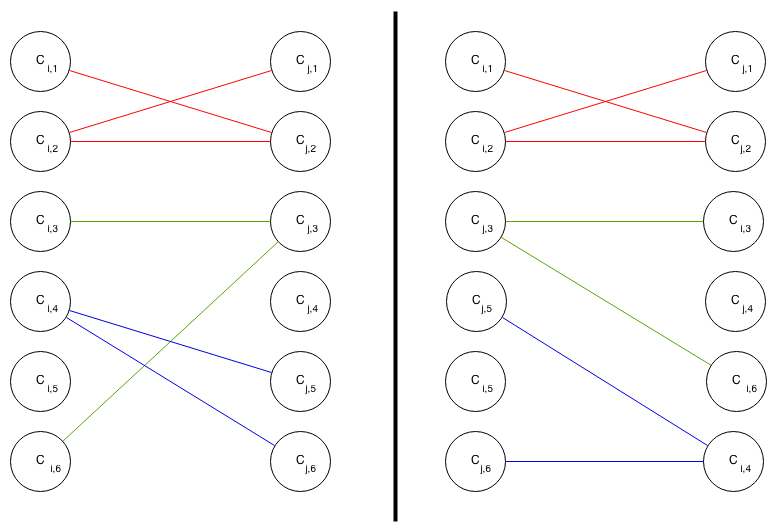
\includegraphics[height=10cm]{kempeSwap.png}\hfill
\centering

$t_i$\hspace{4.5cm}$t_j$\hspace{3.25cm}$t_i$\hspace{4.5cm}$t_j$ \\

\caption{Przykładowa zamiana łańcuchów Kempe: zielonego ($K_d$) i niebieskiego ($K_e$) dla okresów $t_i$ i $t_j$}
\end{figure}

\subparagraph{Przykład} 
Na rysunku powyżej po lewej stronie przedstawiono podgraf $G$, którego wierzchołkami są kursy, których zajęcia zostały przydzielone do okresów $t_i$ i $t_j$, a krawędzie przedstawiają konflikty między tymi kursami. W podgrafie można wyróżnić 5 łańcuchów Kempe: $K_a = \{c_{i1}, c_{i2}, c_{j1}, c_{j2}\}$, $K_b = \{c_{i5}\}$, $K_c = \{c_{j4}\}$, $K_d = \{c_{i3}, c_{i6}, c_{j3}\}$, $K_e = \{c_{i4}, c_{j5}, c_{j6}\}$. Przykładowa zamiana dla łańcuchów $K_d$ i $K_e$ tworzy nowe przypasowanie (na rysunku po prawej stronie) przez przydzielenie $\{c_{i3}, c_{i4}, c_{i6}\}$ do $t_j$ i $\{c_{j3}, c_{i4}, c_{i6}\}$ do $t_i$.

\subparagraph{}Tak określony ruch można traktować jako rozszerzoną wersję podstawowej struktury sąsiedztwa, gdzie zamieniamy po kilka przypasowań na raz. Przy zamianie musimy uważać, aby nie wykonywać ruchów, które powodują przypasowanie do przedziałów czasowych większej liczby kursów, niż jest dostępnych sal. Dodatkowo nakładamy ograniczenia na liczbę kursów biorących udział w zamianie, tj. $|K_1|+ |K_2| \geq 3 $

%- room assignment
\par Po dokonaniu zamian w planie zajęć za pomocą łańcuchów Kempe następuje przypasowanie odpowiedniej sali do poszczególnych zajęć z danego okresu. Sale są przyporządkowywane do kursów metodą zachłanną, w każdym kroku wybieramy kurs, który nie ma przypisanej sali i jest kursem na który uczęszcza najwięcej studentów. Przypisujemy do kursu największą dostępną salę, sala zostaje oznaczona jako niedostępna.

\end{enumerate}
\paragraph{Tabu lista}
służy do przechowywania informacji o zakazanych ruchach, które nie mogą być wykonane przez określoną w tabu tenure dla kursu $c_{i}$ liczbę iteracji.
%-  dokłady opis tabu list
\subparagraph{}W przypadku sąsiedztwa prostego, jeśli zajęcia z kursu $c_i$ zostały przeniesione z okresu $t_j$ i sali $r_k$ w inne miejsce, wtedy przeniesienie jakichkolwiek zajęć z kursu $c_i$ do przedziału czasowego $t_j$ i sali $r_k$ przez kolejne $tt$ iteracji jest ruchem tabu. Podobnie dla sąsiedztwa zaawansowanego, jeśli zajęcia z kursu $c_i$ zostały przeniesione z przedziału czasowego $t_j$ do jakiegoś innego, wtedy przeniesienie jakichkolwiek zajęć z kursu $c_i$ do przedziału czasowego $t_j$ przez kolejne $tt$ iteracji jest ruchem tabu.
\subparagraph{}
Tabu tenure $tt(c_{i})$ obliczane jest na podstawie obecnie uzyskanego rozwiązania oraz częstotliwości przenoszenia zajęć z kursu $c_{i}$ oznaczonej przez $freq(c_{i})$. \\
Tabu tenure wyrażone jest poniższym wzorem: 
 \[tt(c_{i}) = funkcja\ kary\ dla\ obecnego\ rozwiązania + \alpha * freq(c_{i}) \] 
gdzie ${\alpha = \frac{liczba\ konfliktujących\ kursów\ z\ c_{i}}{liczba\ kursów}}$ wobec tego wartość parametru ${\alpha \in [0, 1]}$ \\
gdyż ${liczba\ kursów \geq liczba\ konfliktujących\ kursów\ z\ c_{i}} $

\paragraph{Procedura Tabu Search dla Adaptacyjnego Przeszukiwania Tabu}
\hfill
\begin{algorithm}[H]
    \caption{Algorytm Tabu Search}
    \begin{algorithmic}
    \STATE{$rozwiazanie_{najlepsze} = rozwiazanie_{aktualne}$}
    \WHILE{\emph{nie jest spełniony warunek stopu}}
    \STATE{$rozwiazanie_1 = tabu\_search\_proste\_sasiedztwo(rozwiazanie_{aktualne}, \theta)$}
    \STATE{$rozwiazanie_2 = tabu\_search\_zaawansowane\_sasiedztwo(rozwiazanie_1, \frac{\theta}{3})$}
    \IF	{$jakość(rozwiazanie_2)<jakość(rozwiazanie_{najlepsze})$}
    \STATE $rozwiazanie_{najlepsze} = rozwiazanie_2$
    \STATE $rozwiazanie_{aktualne} = rozwiazanie_2$
    \ENDIF

    \ENDWHILE
    \end{algorithmic}
    \end{algorithm}

\subsubsection{Faza dywersyfikacji}
\par Jeżeli rozwiązanie nie może zostać poprawione za pomocą algorytmu Tabu Search uruchamiana jest trzecia faza - faza dywersyfikacji. Głównym jej elementem jest losowy operator zaburzeń mający na celu zniszczenie osiągniętego lokalnego minimum. Początkowo identyfikowane są zajęcia z wysoką karą wynikającą z funkcji oceny  i losowo wybierane są zajęcia dla których zostaną dokonane zamiany sprecyzowane w poprzedniej fazie.
\par W momencie zakończenia fazy intensyfikacji, poszczególne zajęcia ustawiane są w kolejności malejącej ze względu na wysokość funkcji oceny. Z puli $q$ pierwszych zajęć wybierane jest $n$ zajęć, gdzie zajęcie będące na $k$ miejscu w rankingu wybierane zgodnie z rozkładem prawdopodobieństwa $P(k) = k^{-4.0}$. Następnie dokonywane jest $n$ losowych zamian pomiędzy zajęciami (sprecyzowanych w fazie intensyfikacji), ale tylko takich które zawierają przynajmniej jedno z wybranych z rankingu zajęć. \\
Przykład dla parametrów $q = 5$ i $n = 3$:
\begin{enumerate}
\item Po obliczeniu funkcji kary dla poszczególnych zajęć - ustawiamy zajęcia w kolejności niemalejącej pod względem funkcji kary (w $[\ ]$ podano przykładowe wartości funkcji kary)\\
\begin{enumerate}
 \item[(1)] $(t_{4}, fizyka, sala1)[127]$
 \item[(2)] $(t_{3}, religia, sala1)[89]$
 \item[(3)] $(t_{3}, język\ polski, sala2)[88]$
 \item[(4)] $(t_{4}, etyka, sala2)[80]$
 \item[(5)] $(t_{4}, język\ angielski, sala3)[77]$
 \item[(6)] $(t_{1}, język\ angielski, sala3)[52]$
 \item[(7)] $(t_{1}, biologia, sala2)[40]$
 \item[(8)] $(t_{2}, matematyka, sala2)[34]$
 \item[(9)] $(t_{2}, historia, sala1)[25]$
\end{enumerate}
\item Z puli wszystkich przedmiotów wybieramy $q = 5$ przedmiotów czyli przedmioty $(1) - (5)$ 
\item Rozkłady prawdopodobieństwa dla wybranych $q$ zajęć:
	\begin{enumerate}
	\item[(1)] $P(1) = 1^{-4.0} = 1$
 	\item[(2)] $P(2) = 2^{-4.0} = \frac{1}{16}$
 	\item[(3)] $P(3) = 3^{-4.0} = \frac{1}{81}$
 	\item[(4)] $P(4) = 4^{-4.0} = \frac{1}{256}$
 	\item[(5)] $P(5) = 5^{-4.0} = \frac{1}{625}$
	\end{enumerate}
\item Losowane jest $n = 3$ zajęć zgodnie z powyższym rozkładem prawdopodobieństwa \\
	Przykłady wylosowanych zajęć [*]:
	\begin{enumerate}
	 \item[(1)] $(t_{4}, fizyka, sala1)[127]$
	 \item[(2)] $(t_{3}, religia, sala1)[89]$
	  \item[(4)] $(t_{4}, etyka, sala2)[80]$
	\end{enumerate}
\item Dla każdego z zajęć losujemy typ zamiany: podstawowa zamiana lub Kempe oraz znajdujemy wszystkie wykonywalne zamiany dla tego typu. Losowo wybieramy zamianę i przeprowadzamy ją. Odznaczając zajęcia, które są na liście [*], a dla których została już wykonana zamiana zawierająca te zajęcia.
\end{enumerate}

\subsection{Szczegóły implementacyjne}
\subsubsection{Struktury danych}
\paragraph{} Na potrzeby implementacji algorytmu plan zajęć został zamodelowany przy użyciu podstawowych struktur danych z języka Python. W pierwotnej wersji miał postać słownika, którego kluczami były kolejne numery przedziałów czasowych, a wartościami były listy, które przechowywały obiekty przypasowań zawierające identyfikatory kursu i sali. W trakcie implementacji okazało się, że kopiowanie takiej struktury wymaga korzystania z metody \verb#deepcopy# z modułu \verb#copy#, która przy wielu wywołaniach i dużej strukturze danych okazała się być nieefektywna. Ta obserwacja spowodowała, że w ostatecznej wersji obiekty przypasowań zastąpiono wbudowanym typem \verb#tuple#, co zmniejszyło czas wykonania funkcji kosztu 3-krotnie.
\subsubsection{Funkcja kosztu}
\paragraph{} Pomimo rozbudowanej matematycznej definicji funkcji kosztu w literaturze, efektywna implementacja okazała się być nietrywialna. Pierwsza wersja implementacji potrzebowała przejrzeć cały plan zajęć dla każdego ograniczenia miękkiego, w wersji ostatecznej wystarczą do tego tylko 2 przeglądy. Optymalizacja funkcji kosztu jest kluczowa dla czasu działania algorytmu. Korzystając z narzędzi do profilowania - moduł \verb#line_profile# - zauważyliśmy, że zdecydowaną większość czasu algorytm przeznacza na wykonanie funkcji kosztu.
\subsubsection{Optymalizacje językowe}
\paragraph{} Implementując algorytm staraliśmy się korzystać z funkcjonalnego paradygmatu programowania - funkcji \verb#map# i \verb#filter#, które w porównaniu ze zwykłymi pętlami w Pythonie nie mają dodatkowego narzutu przy iterowaniu. Ponadto korzystanie z elementów programowania funkcjonalnego spowodowało, że kod źródłowy jest w naszej ocenie bardziej zwięzły i czytelny.
\subsubsection{Test-Driven Development}
\paragraph{} Przy implementacji algorytmu staraliśmy wykorzystywać podejście TDD, czyli pisanie testów jednostkowych dla funkcji przed implementacją funkcji. ,,Szczelne'' pokrycie testami jednostkowymi podstawowych funkcji zdecydowanie ułatwiło późniejsze większe zmiany w logice i strukturze algorytmu.


